%%%%%%%%%%%%%%%%%%%%%%%%%%%%%%%%%%%%%%%%%%%%%%
%                insertmeeting
% 1) Title (something creative & funny?)
% 2) Date (MM/DD/YYYY)
% 3) Location (ex. Hagerty High School)
% 4) People/Committees Present 
% 5) Picture 
% 6) Start Time & Stop Time (ex. 12:30AM to 4:30PM)
%%%%%%%%%%%%%%%%%%%%%%%%%%%%%%%%%%%%%%%%%%%%%%
\insertmeeting 
	{Front Wheel Fun} 
	{10/15/21}
	{Hagerty High School}
	{Nathan, Ritam}
	{Images/RobotPics/robot.jpg}
	{2:30 - 4:30}
	
\hhscommittee{Hardware}
\noindent\hfil\rule{\textwidth}{.4pt}\hfil
\subsubsection*{Goals}
\begin{itemize}
    \item Make front wheel assembly
 

\end{itemize} 

\noindent\hfil\rule{\textwidth}{.4pt}\hfil

\subsubsection*{Accomplishments}
After designing the base of our drivetrain yesterday, we started the front wheel assembly. Because we had already CADed one of these for the prototype robot, most of our focus was on creating a way to mount the front wheel. Because it needs to be so tall, we have to create a part that holds the wheel about an inch above the base of the drivetrain and at a 10 degree angle from horizontal. Although this is easy in theory, because we are 3d printing this part and it will be at the front of the robot, where we are most likely to crash, we need to ensure that tis part is a s strong as possible. Before we could start making the main structure of this part, however, we needed to come up with a way to attach it to the rest of the drivetrain. Because we are designing and printing this part separately, we wanted to create a mounting point that is easy to design off of for future design changes. What we decided to make was a small indent in the front of the drive base with a dovetail sticking up (Figure \ref{fig:pic1}). The front wheel assembly will have a corresponding base that will be able to slide onto the rest of the drivetrain. This whole section will be screwed in place to ensure the front wheel doesn't fall off the robot at any time. 
With the dovetail connection point complete, we designed the main structure. It was a challenging task to design something that is so abnormally shaped that still needs to be strong enough to withstand crashes. To strengthen the part we added ribs on the top and bottom that will prevent it from bending and breaking if the robot were to hit a wall (Figure \ref{fig:pic2}). To further strengthen the connection to the rest of the drivetrain, we put holes in the bottom rib that will line up with holes on the drive base (Figure \ref{fig:pic3}). With the part complete, we brought in the wheel assembly from the prototype robot and reassembled it onto the new drivetrain to ensure all of the pieces fit together (Figure \ref{fig:pic4}). We did notice that the bottom ribs were very close to the fork when the wheel turns, so we made a minor adjustment to the shape of the rib.

 

\begin{figure}[ht]
\centering
\begin{minipage}[b]{.48\textwidth}
  \centering
  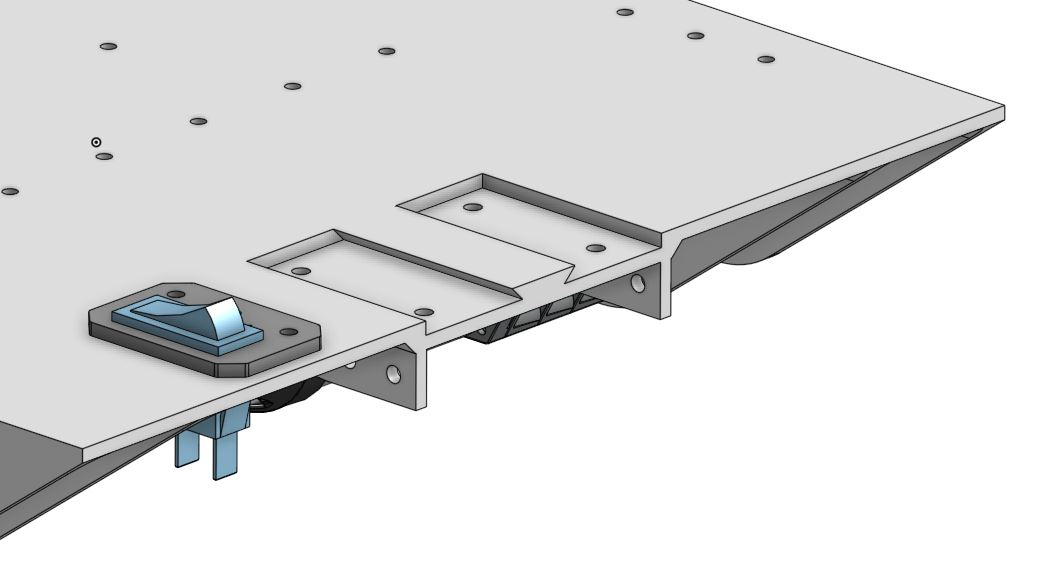
\includegraphics[width=0.95\textwidth]{Meetings/October/10-15-21/10-15-21_CAD_Figure1 - Nathan Forrer.JPG}
  \caption{CAD of the new drivebase.}
  \label{fig:pic1}
\end{minipage}%
\hfill%
\begin{minipage}[b]{.48\textwidth}
  \centering
  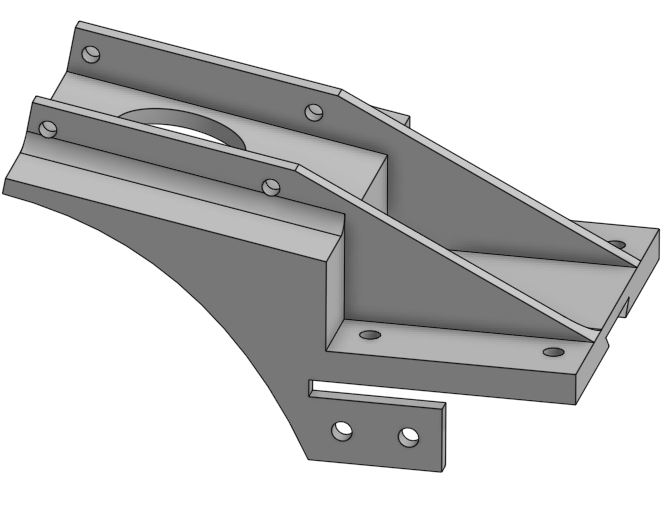
\includegraphics[width=0.95\textwidth]{Meetings/October/10-15-21/10-15-21_CAD_Figure2 - Nathan Forrer.JPG}
  \caption{New ribbing.}
  \label{fig:pic2}
\end{minipage}
\end{figure}

\begin{figure}[ht]
\centering
\begin{minipage}[b]{.48\textwidth}
  \centering
  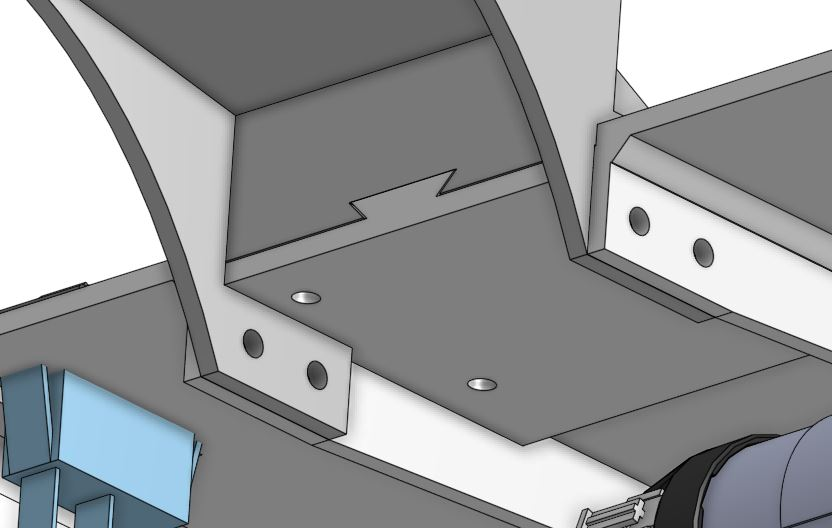
\includegraphics[width=0.95\textwidth]{Meetings/October/10-15-21/10-15-21_CAD_Figure3 - Nathan Forrer.JPG}
  \caption{Strengthening the connection.}
  \label{fig:pic3}
\end{minipage}%
\hfill%
\begin{minipage}[b]{.48\textwidth}
  \centering
  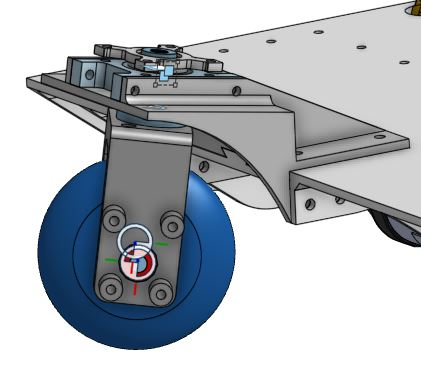
\includegraphics[width=0.95\textwidth]{Meetings/October/10-15-21/10-15-21_CAD_Figure4 - Nathan Forrer.JPG}
  \caption{The current assembly.}
  \label{fig:pic4}
\end{minipage}
\end{figure}

\whatsnext{
\begin{itemize}
    \item Print drivetrain
    \item Assemble drivetrain
\end{itemize} 
}

